\section{Hybrid Job Placement}
\label{sec: hybrid placement}

Based on our experiments with two workloads, the ``bullying" is inevitable when the dragonfly network is configured with random placement and (progressive) adaptive routing. 
The precaution to stop the ``bullying" is to avoid network sharing between concurrently running jobs, 
and contiguous placement and minimal routing could be an effective way. 
However, the network would suffer severe local congestion and unbalanced utilization when contiguous placement and minimal routing is in use. 
Running each job with dedicated routing policy is unrealistic, 
since routing policy is part of system configuration which can not be changed on the fly upon job submission. 
Assigning preferable allocation to each job based on its communication intensity is applicable for the batch scheduler with intelligent job placement policy. 



We propose a hybrid job placement policy to assign each job with preferable allocation. 
According to the hybrid placement policy, 
the less communication-intensive jobs get contiguous allocation to partially avoid network sharing with the ``bully", 
while the communication-intensive jobs get random allocation in order to share network resource with each other. 
When Workload~\Rmnum{1} is running on the dragonfly network with hybrid placement policy, 
AMG gets contiguous allocation, MultiGrid and CrystalRouter get random allocations. 
The experiment results show that hybrid placement performs comparably as random placement for improving network performance and mitigates the degradation of AMG caused by the ``bullying".
\footnote{Due to page limit, we won't present the analysis about network traffic and saturated time in this section.}



\subsection{Network Performance Analysis}

Hybrid placement is also coupled with three routing policies, Minimal, Adaptive and Progressive Adaptive. They are denoted respectively as HM, HA and HPA. As presented in the previous section, random placement outperforms contiguous placement in terms of network performance, we only compare the results of hybrid placement with random placement due to the page limit.


\begin{table}[ht]
\begin{center}
\caption{Average time spent on communication by all MPI ranks when Workload I is running on dragonfly network under hybrid placement and random placement policies.} 
\label{tab: hyb-placement-wkld-commtime}
\begin{tabular}{l c c c c c c }
\toprule % Top horizontal line
\toprule
&\multicolumn{6}{c}{Placement and Routing Configurations} \\
\cmidrule(l){2-7}
          & HM & HA & HPA & RM & RA & RPA \\ % Column names row
\midrule % In-table horizontal line
Time(ms)  &273 &255 &255 &255 &265 &264  \\ % Content row 1
%\midrule
%Workload II &1747 &1991 &1991 &1791 &2367 &1965 \\
\midrule % In-table horizontal line
\bottomrule % Bottom horizontal line
\end{tabular}
\end{center}
\end{table}


As shown in Table \ref{tab: hyb-placement-wkld-commtime}, hybrid placement and random placement perform comparably. When coupled with minimal routing, RM outperforms HM. However, when coupled with (progressive) adaptive routing, HA and HPA outperform RA and RPA. HA and HPA perform equally well as compared with RM.  


\subsection{Individual Application Analysis}

\begin{figure*}[t!]
    \centering
    \begin{subfigure}[t]{0.32\textwidth}
        \centering
        \includegraphics[height=1.3 in]{hyb-plcmt/amg/commtime}
        \caption{AMG Communication Time}
        \label{fig:hyb-plcmt-amg-commtime}
    \end{subfigure}\hfill
    \hspace{1em}%
    \begin{subfigure}[t]{0.32\textwidth}
        \centering
        \includegraphics[height=1.3 in]{hyb-plcmt/mg/commtime}
        \caption{MG Communication Time}
        \label{fig:hyb-plcmt-mg-commtime}
    \end{subfigure}\hfill
    \begin{subfigure}[t]{0.32\textwidth}
        \centering
        \includegraphics[height=1.3 in]{hyb-plcmt/cr/commtime}
        \caption{CR Communication Time}
        \label{fig:hyb-plcmt-cr-commtime}
    \end{subfigure}%
   \caption{Application communication time. Workload \Rmnum{1} is running under all the possible placement and routing configurations.}
   \label{fig:hyb-plcmt-apps-commtime}
\end{figure*}

Figure \ref{fig:hyb-plcmt-apps-commtime} shows the communication time of each application when hybrid placement configurations are in use. MultiGrid and CrystalRouter have basically the same performance with hybrid placement as compared with random placement. Since they still get random allocation in the hybrid placement. The performance of AMG is significantly improved when hybrid placement is in use. Compared with ``RA" and ``RPA", ``HA" and ``HPA" can greatly reduce AMG communication time, shown in Figure \ref{fig:hyb-plcmt-amg-commtime}. This is due the contiguous allocation assigned to AMG in the hybrid placement policy. When being coupled with minimal routing, hybrid placement and contiguous placement have similar performance for AMG. However, when (progressive) adaptive routing are in use, the traffic from MultiGrid and CrystalRouter still might be redirected to the routers serving AMG. Since AMG is less communication-intensive and can not fully utilize network, it is likely that the intermediate routers picked for the traffic from MultiGrid and CrystalRouter could be from AMG's groups. So for AMG, ``HA" and ``HPA" are worse than ``CA" and ``CPA", but they are much better than ``RA" and ``RPA".

\subsection{Key Observations}

Based on the results from experimenting with hybrid placement policy, we can make the following observations.

\emph{Compared with random placement policy, hybrid placement can guarantee comparable network performance.} Hybrid placement policy allows network sharing between communication intensive applications, thus alleviates the potential congestion and improves network utilization.

\emph{Hybrid placement can mitigate the performance degradation of less communication-intensive application.} Hybrid placement policy preserves contiguous allocation for less communication-intensive application, prevents network resource from being shared by others. Unlike random placement indulging the ``bully", hybrid placement can restrain it to some extent.

Hybrid placement can guarantee the performance of individual application without causing performance degradation to network performance. Compared with contiguous and random placement policy, hybrid placement are more preferable to HPC systems with dragonfly networks.


